\documentclass[tikz,border=8pt]{standalone}
% Shared look for every TikZ diagram. Load with % Shared look for every TikZ diagram. Load with % Shared look for every TikZ diagram. Load with \input{../../tools/tikz-style.tex}
\usepackage[T1]{fontenc}
\usepackage{lmodern}
\renewcommand{\sfdefault}{lmr}  % diagrams use the same serif as the text
\usetikzlibrary{arrows.meta, positioning, shapes.geometric, calc, fit, backgrounds}
\definecolor{cblue}{HTML}{4C78A8}
\definecolor{corange}{HTML}{F58518}
\definecolor{cgreen}{HTML}{54A24B}
\definecolor{cred}{HTML}{E45756}
\definecolor{cpurple}{HTML}{B279A2}
\definecolor{cgrey}{HTML}{6B6B6B}
\tikzset{
  every picture/.style={font=\sffamily, line width=1.2pt},
  box/.style={draw=#1, fill=#1!12, rounded corners=4pt, align=center, inner sep=7pt, minimum height=1.1cm},
  box/.default=cgrey,
  arrow/.style={-{Stealth[length=3mm]}, draw=cgrey, line width=1.4pt},
  title/.style={font=\sffamily\bfseries\Large},
  note/.style={font=\sffamily\small, text=cgrey, align=center},
}
\AtBeginDocument{\hyphenpenalty=10000 \exhyphenpenalty=10000}

\usepackage[T1]{fontenc}
\usepackage{lmodern}
\renewcommand{\sfdefault}{lmr}  % diagrams use the same serif as the text
\usetikzlibrary{arrows.meta, positioning, shapes.geometric, calc, fit, backgrounds}
\definecolor{cblue}{HTML}{4C78A8}
\definecolor{corange}{HTML}{F58518}
\definecolor{cgreen}{HTML}{54A24B}
\definecolor{cred}{HTML}{E45756}
\definecolor{cpurple}{HTML}{B279A2}
\definecolor{cgrey}{HTML}{6B6B6B}
\tikzset{
  every picture/.style={font=\sffamily, line width=1.2pt},
  box/.style={draw=#1, fill=#1!12, rounded corners=4pt, align=center, inner sep=7pt, minimum height=1.1cm},
  box/.default=cgrey,
  arrow/.style={-{Stealth[length=3mm]}, draw=cgrey, line width=1.4pt},
  title/.style={font=\sffamily\bfseries\Large},
  note/.style={font=\sffamily\small, text=cgrey, align=center},
}
\AtBeginDocument{\hyphenpenalty=10000 \exhyphenpenalty=10000}

\usepackage[T1]{fontenc}
\usepackage{lmodern}
\renewcommand{\sfdefault}{lmr}  % diagrams use the same serif as the text
\usetikzlibrary{arrows.meta, positioning, shapes.geometric, calc, fit, backgrounds}
\definecolor{cblue}{HTML}{4C78A8}
\definecolor{corange}{HTML}{F58518}
\definecolor{cgreen}{HTML}{54A24B}
\definecolor{cred}{HTML}{E45756}
\definecolor{cpurple}{HTML}{B279A2}
\definecolor{cgrey}{HTML}{6B6B6B}
\tikzset{
  every picture/.style={font=\sffamily, line width=1.2pt},
  box/.style={draw=#1, fill=#1!12, rounded corners=4pt, align=center, inner sep=7pt, minimum height=1.1cm},
  box/.default=cgrey,
  arrow/.style={-{Stealth[length=3mm]}, draw=cgrey, line width=1.4pt},
  title/.style={font=\sffamily\bfseries\Large},
  note/.style={font=\sffamily\small, text=cgrey, align=center},
}
\AtBeginDocument{\hyphenpenalty=10000 \exhyphenpenalty=10000}

\begin{document}
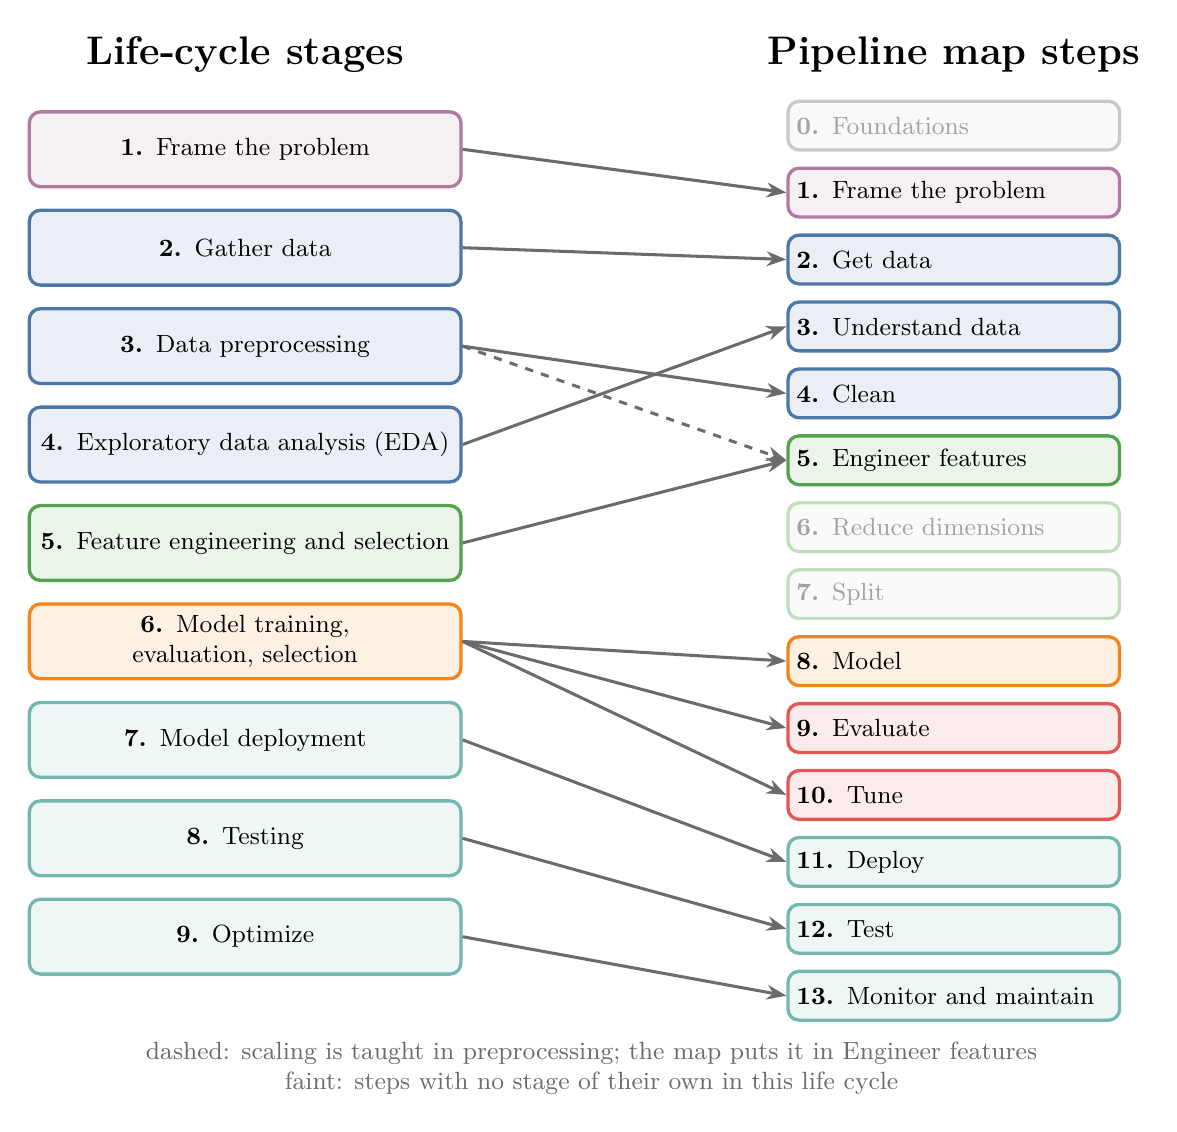
\begin{tikzpicture}
  \definecolor{cteal}{HTML}{72B7B2}
  \tikzset{st/.style={box=#1, minimum width=5.4cm, text width=5.2cm, minimum height=0.95cm, inner sep=4pt, font=\small},
           ps/.style={box=#1, minimum width=4.2cm, text width=4.0cm, minimum height=0.62cm, inner sep=3pt, font=\small, align=left},
           link/.style={draw=cgrey, line width=1.1pt, -{Stealth[length=2.5mm]}},
           part/.style={link, dashed}}
  \node[title] at (0,0.9) {Life-cycle stages};
  \node[title] at (9,0.9) {Pipeline map steps};
  % the 14 Pipeline map steps (right); steps no stage maps to are faint
  \foreach \k/\t/\c/\o in {0/Foundations/cgrey/0.35, 1/Frame the problem/cpurple/1, 2/Get data/cblue/1, 3/Understand data/cblue/1,
      4/Clean/cblue/1, 5/Engineer features/cgreen/1, 6/Reduce dimensions/cgreen/0.35, 7/Split/cgreen/0.35, 8/Model/corange/1,
      9/Evaluate/cred/1, 10/Tune/cred/1, 11/Deploy/cteal/1, 12/Test/cteal/1, 13/Monitor and maintain/cteal/1}
    \node[ps=\c, opacity=\o, text opacity=\o] (p\k) at (9,{-0.85*\k}) {\textbf{\k.} \t};
  % the 9 stages (left), in the order taught
  \foreach \i/\t/\c in {1/Frame the problem/cpurple, 2/Gather data/cblue, 3/Data preprocessing/cblue,
      4/Exploratory data analysis (EDA)/cblue, 5/Feature engineering and selection/cgreen,
      6/{Model training, evaluation, selection}/corange, 7/Model deployment/cteal, 8/Testing/cteal, 9/Optimize/cteal}
    \node[st=\c] (s\i) at (0,{-0.3-1.25*(\i-1)}) {\textbf{\i.} \t};
  \foreach \a/\b in {1/1, 2/2, 3/4, 4/3, 5/5, 6/8, 6/9, 6/10, 7/11, 8/12, 9/13} \draw[link] (s\a.east) -- (p\b.west);
  \draw[part] (s3.east) -- (p5.west);
  \node[note, anchor=north] at (4.4,-11.5) {dashed: scaling is taught in preprocessing; the map puts it in Engineer features\\faint: steps with no stage of their own in this life cycle};
\end{tikzpicture}
\end{document}
